\documentclass[a4paper,10pt]{report}
\usepackage[T1]{fontenc}
\usepackage[table]{xcolor}
\usepackage{titlesec}
\usepackage{graphicx}
\usepackage[inkscapepath=../assets/svg]{svg}
\usepackage{amsmath}
\usepackage{amsthm}
\usepackage{mathtools}
\usepackage{fancyvrb}
\usepackage[english]{babel}
\usepackage{csquotes}
\usepackage{hyperref}
\hypersetup{
   colorlinks=true,
   linkcolor=blue,
   urlcolor=cyan
}
\usepackage{tikz}
\usepackage{amssymb}
\usepackage[sc]{mathpazo}
\linespread{1.05}
\usepackage{microtype}
\usepackage{breqn}
\usepackage{caption}
\usepackage{subcaption}
\usepackage[
   backend=bibtex,%
   bibencoding=utf8,%
   language=english,%
   style=numeric-comp,%
   sorting=nyt,%
   maxbibnames=10,%
   natbib=true%
]{biblatex}
\addbibresource{references.bib}
\usepackage{siunitx}
\usepackage{booktabs}
\usepackage{longtable}
\usepackage{geometry}
\usepackage{multirow}
\graphicspath{ {../assets/img/} }

\newgeometry{hmargin={30mm,30mm}}

% Set TOC depth and sections numbering
\setcounter{tocdepth}{3}
\setcounter{secnumdepth}{3}

% Remove chapters head and reduce spacing
\titleformat{\chapter}[hang]{\Large\bfseries}{\thechapter \hspace{2ex}}{0pt}{\Large}
\titlespacing{\chapter}{0cm}{0cm}{0.5cm}
\usepackage[parfill]{parskip}

% Make quotes italic
\renewcommand{\mkbegdispquote}[2]{\itshape}

% Change texttt line breaks
\renewcommand{\texttt}[1]{%
  \begingroup
  \ttfamily
  \begingroup\lccode`~=`.\lowercase{\endgroup\def~}{.\discretionary{}{}{}}%
  \catcode`/=\active\catcode`[=\active\catcode`.=\active
  \scantokens{#1\noexpand}%
  \endgroup
}


\begin{document}
\frenchspacing

% First page
\title{
	{{\large{\textsc{Alma Mater Studiorum $\cdot$ University of Bologna}}}}
	\rule{\textwidth}{0.4pt}\vspace{3mm}
	\textbf{Question answering on the SQuAD dataset}
	\begin{figure}[!htb]
		\centering
		
\includegraphics[width = 100pt]{squad-logo}
	\end{figure} \\
	NLP course final project
}

\author{Leonardo Calbi (\href{mailto:leonardo.calbi@studio.unibo.it}{leonardo.calbi@studio.unibo.it}) \\ Lorenzo Cellini (\href{mailto:lorenzo.cellini3@studio.unibo.it}{lorenzo.cellini3@studio.unibo.it}) \\ Alessio Falai (\href{mailto:alessio.falai@studio.unibo.it}{alessio.falai@studio.unibo.it})}
\date{\today}
\maketitle
\newpage
\tableofcontents
\setcounter{tocdepth}{1}
%\listoffigures
%\listoftables
\newpage


\chapter{Summary}\label{chap:introduction}

The tasks of machine comprehension (MC) and question answering (QA) have gained significant popularity over the past few years within the natural language processing and computer vision communities. Systems trained end-to-end now achieve great results on a variety of tasks in the text and image domains.

In this work we address a question answering problem and, in particular, the Stanford Question Answer Dataset (SQuAD) problem: given a large collection of Wikipedia articles with associated questions, the goal is to identify the span of characters that contains the answer to the question.

This project focuses on the SQuAD v1.1 dataset, that contains more than 100,000 question-answer pairs on more than 500 articles. Here each question has at least one associated answer, whereas in the SQuAD v2.0 dataset there are also questions with no answers at all.

In this work we implement and compare five different models: 
\begin{itemize}
  \item a naïve LSTM encoder-decoder that will act as our baseline;
  \item the Bi-Directional Attention Flow (BIDAF) network (CITAZIONE);
  \item a model that wraps a pretrained Bidirectional Encoder Representations from Transformers (BERT), as language model, coupled with a custom output layer on top of it;
  \item a model that wraps DistilBERT, a smaller general-purpose language representation model, 40\% smaller then BERT but with 97\% of its language understanding capabilities and 60\% faster;
  \item a model that wraps ELECTRA, a more sample-efficient pre-training task called "replaced token detection".

\end{itemize}
For the last three models, we developed a modular reusable output layer, allowing us to implement different models by only change the language model levels (input, embedding and modelling).

Our experimental evaluations show that our models achieve …………………………………………….

\chapter{Background}\label{chap:background}

As already described above, the question answering task is based on the idea of identifying one possible answer to the given question as a subset of the given context. 

Since the input data is of textual form and the latest models for the task are all based on neural architectures, there is the need to encode such text into a numeric representation. As of today, there are two main approaches to embed words in numerical format: sparse embeddings, like TF-IDF \cite{tf-idf} and PPMI \cite{ppmi}, and the modern dense embeddings, such as Word2Vec \cite{word2vec} and GloVe \cite{glove}. In the latter case, embeddings for each word in the input vocabulary are usually computed with shallow encoders. 

These emebddings are then used as inputs for models specialized in processing sequential inputs. Nowadays, such models are mostly based on the Transformer architecture \cite{transformers}, which has the attention mechanism at its core. Instead, before this revolution, NLP competition's leaderboards were mostly populated by models based on recurrent and convolutional modules.

The most influential recurrent networks are LSTMs \cite{lstm} and GRUs \cite{gru}. They are both based on processing sequential inputs and they keep an evolving series of hidden states, such that the output $h_t^{(0)}$ is a function of $h_{t-1}^{(0)}$ and the input $x_t$ at position $t$. Recurrent layers can also be stacked to increase the capacity of the network: in that case, $h_t^{(0)}$ would act as an input to $h_t^{(1)}$, i.e. the first hidden state of the next depth-wise layer, and the same goes for the successive layers, as shown in figure \ref{fig:recurrent}.

\begin{figure}[h]
    \center
    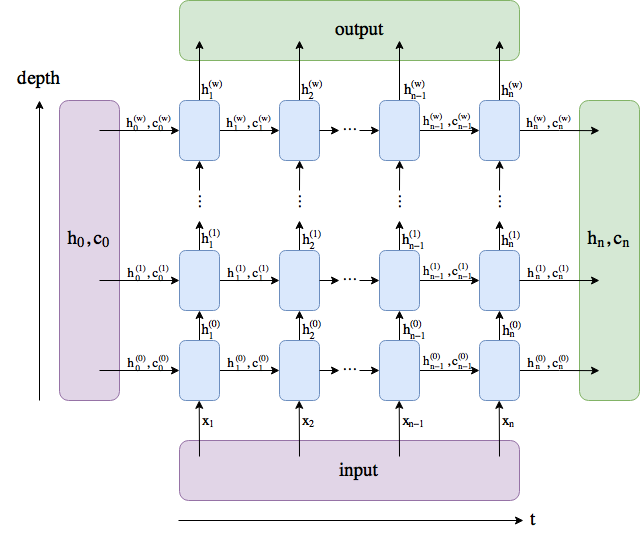
\includegraphics[width=0.65\linewidth]{recurrent}
    \caption{Recurrent module (image courtesy of \cite{recurrent-img})}
    \label{fig:recurrent}
\end{figure}

In natural language, meaning does not usually simply flow from left to right, so that in RNNs other techniques may be necessary to reach a higher level of understanding. One example of such improvement is bi-directionality: the input is processed in two ways, from left to right (the "forward" pass) and from right to left (the "backward" pass); then, outputs of the two computations are merged together (usually by concatenating them over their last dimension). The intuition behind bi-directional RNNs is that they tend to understand the overall context better than their uni-directional counterparts, since they are able to aggregate information from the "past" and from the "future".

About Transformers, at a high-level, they comprise a stack of encoder-decoder modules, where each encoder features a multi-head attention block (to focus on different subsets of the input sequence when encoding one specific token) and a point-wise fully-connected layer, while each decoder features the same architecture as the encoder, but with an additional multi-head attention block in the middle (that helps the decoder focus on relevant parts of the input sequence).

The multi-head attention modules in the Transformer architecture are the ones responsible for gathering information from other tokens in the input sequence, thus resembling the task of hidden states in RNNs (i.e. incorporate the representation of previous inputs with the currently processed one).

\begin{figure}[h]
    \center
    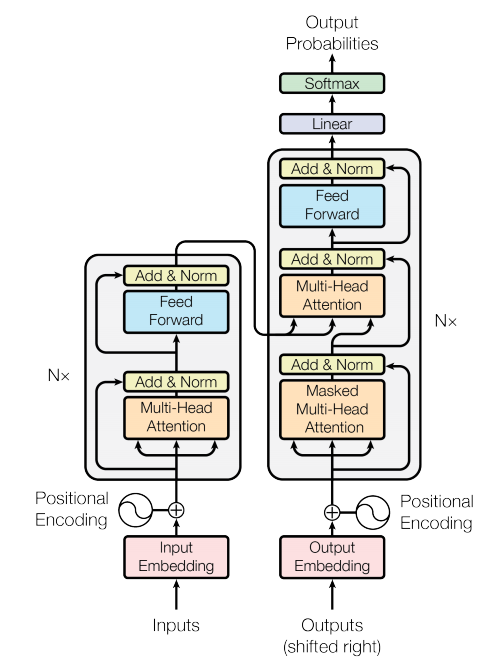
\includegraphics[width=0.45\linewidth]{transformers}
    \caption{Transformers (image taken from \cite{transformers})}
    \label{fig:transformers}
\end{figure}

While Transformers may always seem the way to go, since they throw away all the computational burden of training recurrent modules (which are sequential in nature and, thus, scarcely parallelizable), they also suffer from limitations due to the quadratic complexity of attention and the inherent maximum number of input tokens (which is implicitly linked to architecture choices themselves).


\chapter{System description}\label{chap:system-description}

In this work we implement three distinct models: a naïve LSTM encoder-decoder that will act as our baseline, the Bi-Directional Attention Flow (BIDAF) network (CITAZIONE) and a model that wraps a pretrained Bidirectional Encoder Representations from Transformers (BERT), as language model, coupled with a custom output layer on top of it.

Each model is trained on the SQuAD v1.1 training set and evaluated on the SQuAD v1.1 dev set, available on the github repository of the SQuAD project (link).

The models’ evaluation is carried out on the same preprocessed data: indeed, we defined a preprocessing pipeline, applied it to the training and dev set once and the resulting dataset is fed to each model. (CONTROLLARE QUI – mi pare che per bert abbiamo tokenizzato diversamente)

In order to perform an effective models’ comparison, each model shares the same input and output layer: what changes is the language model (embedding + attention layers) and the modelling layer.

The following is a detailed description of the models.

\section{Baseline}\label{sec:baseline}

….

\section{BiDAF}\label{sec:bidaf}

Sintesi tra paper bidaf e medium

\section{BERT}\label{sec:bert}

….

\chapter{Experimental setup and results}\label{chap:experiments}

\section{Data handling}
Given the JSON training set, we decided to parse it into a suitable tabular data structure, which turned to be useful even for subsequent pre-processing tasks. In particular, since each context has multiple question/answer pairs and each question can have multiple answers, we allocated one row for each context/question/answer triple, thus replicating the same context and question multiple times, in order to consider it as a separate example.

Regarding the splitting strategy for the dataset, we went for a simple holdout, thus setting aside $20\%$ of the whole dataset for validation purposes. The way the validation set is built guarantees that the entire set of rows referencing to the same context is kept into the same split, thus avoiding unjustifiable boosting of results.

As an additional test, we evaluated all of our models on the official SQuAD v1.1 dev set. The main difference between this dataset and the training one is that the same question can have multiple correct answers.

\section{Tokenization}
Tokenization has the following meaning: given a string of text, its task is to split it into sub-strings (called tokens), depending on the chosen algorithm. Different models call for different tokenization pipelines. In our case, we have two macro-categories:
\begin{enumerate}
  \item Recurrent-based models tokenizer: splits words by whitespaces and punctuations, removes accents and applies a lowercasing function to all the tokens. Moreover, questions are padded (not truncated), while contexts are truncated and padded. Taking inspiration from \cite{max-context-tokens}, the maximum number of tokens for truncating contexts was fixed to $300$. 
  \item Transformer-based models tokenizer: splits words using the WordPiece algorithm (introduced in \cite{wordpiece}), removes accents and applies a lowercasing function to all the tokens, while also merging together questions and contexts as $[CLS] q_1 q_2 \dots q_n [SEP] c_1 c_2 \dots c_m [SEP]$ (it leverages the special tokens $[CLS]$ and $[SEP]$). Moreover, the combined question/context sentence is truncated to a maximum number of tokens ($512$, as in \cite{bert}) and padded to the right.
\end{enumerate} 
Tokenization happens on the fly at the batch level, thus enabling us to perform dynamic padding (based on the longest sequence in a batch) and avoiding the pre-tokenization overhead.

The tokenizer is also used as some kind of pre-processor, to remove from the training dataset those rows whose contexts would not contain the relative answer, after truncation. 

\section{Embeddings}
In recurrent-based models, tokens are numerically encoded using the standard GloVe embeddings. In particular, we tested different types of GloVe models, with different embedding dimensions:
\begin{itemize}
  \item Wikipedia 2014 and Gigaword 5 (6B tokens, 400K vocab, uncased, 300d vectors)
  \item Twitter (2B tweets, 27B tokens, 1.2M vocab, uncased, 200d vectors)
\end{itemize}

We additionally embedded two more tokens (not present in the standard GloVe vocabulary):
\begin{enumerate}
  \item $[PAD]$: the corresponding vector contains all zeros
  \item $[UNK]$: the corresponding vector, which is used to handle OOV (Out Of Vocabulary) words, is the mean of all the GloVe vectors, as reported by Pennington (one of GloVe's authors) 
  \begin{displayquote}I've found that just taking an average of all or a subset of the word vectors produces a good unknown vector \end{displayquote}
\end{enumerate}

In Transformer-based models, we instead rely on the wrapped language models of the HuggingFace library \cite{hugginface}, so that there is no need to manually handle token embeddings.

\section{Metrics}
Models are evaluated at the end of each epoch and metrics are computed for both the training and validation set. In our case, the validation set was mainly used to track models' performance on unseen data, in order to avoid overfitting problems.

Metrics used for evaluating the models are F1 and EM (Exact Match) and they were taken from the official SQuAD evaluation script. The F1 score ($f1=\frac{2\cdot p \cdot r}{p+r}$), defined as the harmonic mean between precision ($p=\frac{TP}{TP+FP}$) and recall ($r=\frac{TP}{TP+FN}$), is computed per question and then averaged across all questions. The EM score is instead computed as the number of questions that are answered in exact same words as the ground truth, divided by the total number of questions.

Since the same question can have multiple ground truths (specifically, in the dev set), there is the need to select just one for each question. To fulfill this requirement, only the nearest ground truth for each prediction is considered: given a prediction $p=[p_s, p_e]$, where $p_s$ is the start index of the predicted answer and $p_e$ is the corresponding end index, and a set of associated ground truths $G=\{[g_s^{(0)},g_e^{(0)}], \dots, [g_s^{(n)},g_e^{(n)}]\}$, the selected ground truth is $\min_{g\in G}\Vert p - g\Vert_2$. 

Moreover, we noticed that the training set does not have multiple answers for the same question, so this "nearest answer" approach comes into play only at inference time: this is actually the desired behavior, since at training time the described technique could lead to an unstable learning process, given by the non-stationarity of the target distribution.

\section{Environment}
The main third-party libraries on which the project is based on are PyTorch \cite{pytorch}, an open source machine learning framework with automatic differentiation and eager execution, and HuggingFace \cite{hugginface}, a library to build, train and deploy state of the art NLP models.

All of the training and validation processes were executed on Google Colaboratory \cite{colab}, a platform that gives the possibility to exploit some computational resources for free. In particular, Colab allows you to select a GPU runtime, that boosts the training time of neural models and most of the times we were assigned an NVIDIA Tesla T4 GPU, with 16GB of RAM. 

Training and evaluation metrics, along with model checkpoints and results, are directly logged into a W\&B project \cite{wandb}, which is openly accessible \href{https://wandb.ai/wadaboa/squad-qa}{here}.

\section{Results}

\begin{table}[h]
  \center
  \begin{tabular}{|c|c|c|c|c|c|c|}
  \hline
  \multirow{2}{*}{}   & \multicolumn{2}{c|}{\textbf{Training}} & \multicolumn{2}{c|}{\textbf{Validation}} & \multicolumn{2}{c|}{\textbf{Test}} \\ \cline{2-7} 
                      & \textbf{F1}        & \textbf{EM}       & \textbf{F1}         & \textbf{EM}        & \textbf{F1}      & \textbf{EM}     \\ \hline
  \textbf{Baseline}   &                    &                   &                     &                    &                  &                 \\ \hline
  \textbf{BiDAF}      &                    &                   &                     &                    &                  &                 \\ \hline
  \textbf{BERT}       &                    &                   &                     &                    &                  &                 \\ \hline
  \textbf{DistilBERT} &                    &                   &                     &                    &                  &                 \\ \hline
  \textbf{ELECTRA}    &                    &                   &                     &                    &                  &                 \\ \hline
  \end{tabular}
  \caption{Results}
  \label{table:results}
\end{table}

\chapter{Analysis of results}\label{chap:analysis-results}

\chapter{Discussion}\label{chap:discussion}

\printbibliography

\end{document}
